\iffabian
\else
	\subsection{Integration des Profils in die Benutzeroberfläche}
\fi

Sobald C Compact mit einem Profil geöffnet wurde, wird auf der rechten Seite ein zusätzlicher Tab eingeblendet, bei welchem vom Benutzer auf die Profilinformationen zugegriffen werden kann. Hier findet der Nutzer Nutzernamen, Profilbild und die Errungenschaften, welche er bis jetzt bekommen hat.

\begin{figure}[h] 
  \centering
     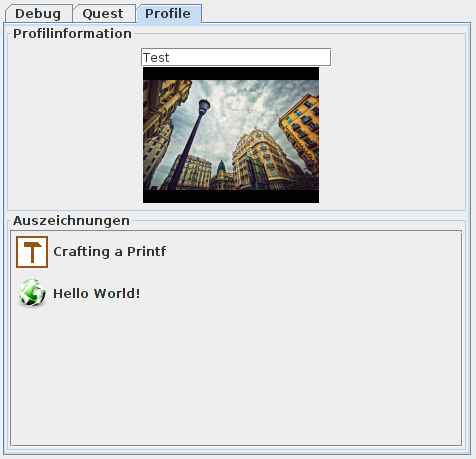
\includegraphics[width=0.7\textwidth]{./media/images/gui/profile.png}
  \caption{Integration des Profiles im GUI}
  \label{fig:profile_gui}
\end{figure}


Mit einem einfach Klick auf das Feld in dem der Benutzername steht, kann dieser geändert werden. Der neue Name wird gespeichert sobald das Textfeld den Fokus verliert oder die Entwicklungsumgebung von C Compact geschlossen wird.

Das Profilbild kann verändert werden, indem man auf das aktuelle, bereits vorhandene klickt. Nun öffnet sich ein JFileChooser. In diesem kann das gewünschte Bild ausgewählt werden, welches dann auf der rechten Seite des Frames zu sehen ist. Weiters wird auch der Bildname eingeblendet. Mit einem einfachen Klick auf den Button "`Öffnen"', wird das Bild vom Programm übernommen und im Profil gespeichert und in der Folge automatisch auf die im Programm definierte Größe angepasst.

Wenn ein defektes Bild gewählt wurde, wird im Profil mithilfe eines Schriftzuges darauf hingewiesen. Das defekte Profilbild kann wiederum mithilfe eines Klicks auf den Schriftzug ausgewechselt werden.

Zur Anzeige der Auszeichnungen wird eine JScrollpane verwendet, die Anzahl der Auszeichnungen, welche angezeigt werden kann, ist somit nicht begrenzt. Sichtbar sind das Bild und der Titel der Auszeichnung. Wenn man mit dem Mauszeiger eine gewisse Zeit lang über einem Token stehen bleibt, erscheint ein kleines Popup, welches eine in html-codierte Beschreibung enthält.

Zur Hilfestellung wurden Tooltips\footnote{\url{https://docs.oracle.com/javase/tutorial/uiswing/components/tooltip.html}} eingefügt, welche Benutzer im Programm helfen sollen. Diese zeigen an, wie man sein Profilbild und den Namen ändern kann. Sie werden sichtbar, wenn man mit dem Mauszeiger über die eingestellten Fenster fährt.